\documentclass[12pt,a4paper]{report}
\usepackage[utf8]{inputenc}
\usepackage[margin=1in]{geometry}
\usepackage{graphicx}
\usepackage{listings}
\usepackage{xcolor}
\usepackage{booktabs}
\usepackage{hyperref}
\usepackage{fancyhdr}
\usepackage{amsmath}
\usepackage{longtable}

\hypersetup{
    colorlinks=true,
    linkcolor=blue,
    filecolor=magenta,      
    urlcolor=cyan,
    pdftitle={Edusoft - Technical Report},
    pdfpagemode=FullScreen,
}

\definecolor{codegreen}{rgb}{0,0.6,0}
\definecolor{codegray}{rgb}{0.5,0.5,0.5}
\definecolor{codepurple}{rgb}{0.58,0,0.82}
\definecolor{backcolour}{rgb}{0.95,0.95,0.92}

\lstdefinestyle{mystyle}{
    backgroundcolor=\color{backcolour},   
    commentstyle=\color{codegreen},
    keywordstyle=\color{magenta},
    numberstyle=\tiny\color{codegray},
    stringstyle=\color{codepurple},
    basicstyle=\ttfamily\footnotesize,
    breakatwhitespace=false,         
    breaklines=true,                 
    captionpos=b,                    
    keepspaces=true,                 
    numbers=left,                    
    numbersep=5pt,                  
    showspaces=false,                
    showstringspaces=false,
    showtabs=false,                  
    tabsize=2
}
\lstset{style=mystyle}

\pagestyle{fancy}
\fancyhf{}
\rhead{Edusoft Technical Report}
\lhead{HCMIU - Web Application Development}
\cfoot{\thepage}

\begin{document}

\begin{titlepage}
    \begin{center}
        \vspace*{1cm}
        
        \Huge
        \textbf{Edusoft}
        
        \vspace{0.5cm}
        \LARGE
        Comprehensive School Management System
        
        \vspace{1.5cm}
        \Large
        \textbf{Technical Report}
        
        \vspace{0.8cm}
        \large
        Course: Web Application Development (25\% of Grade)\\
        International University - VNU-HCM
        
        \vfill
        
        \textbf{Team Members:}\\
        \begin{tabular}{ll}
            Tran Anh Van & ITITWE22171 \\
            Nguyen Tran Minh Thu & ITITWE24025 \\
        \end{tabular}
        
        \vspace{1.5cm}
        
        \includegraphics[width=0.25\textwidth]{UseCaseDiagram.png} % Fallback or placeholder for university logo/project logo
        
        \vfill
        
        \large
        Date: June 3, 2026
        
    \end{center}
\end{titlepage}

\tableofcontents
\listoffigures
\listoftables

\chapter{Executive Summary}
\section{Project Overview}
Edusoft is a comprehensive, production-grade School Management System (SMS) built to streamline administration and academic registry operations at the university level. Academic institutions frequently grapple with disparate administrative systems, manual registrar validations, and latency in academic advisor sign-offs. Edusoft addresses these operational challenges by consolidating key workflows under a unified, role-based single-page application (SPA).

\section{Problem Statement}
In traditional academic environments, student registration, financial ledger adjustments, and advising approvals operate as disconnected systems. This isolation introduces manual inefficiencies, such as advisors reviewing course requests without real-time schedule conflict checks or credit caps. Furthermore, delayed tuition invoice generation leads to non-compliant student enrollments. Edusoft resolves these operational bottlenecks through a reactive, transaction-safe database model that enforces constraints at the engine level.

\section{Target User Groups}
The application supports three primary user groups, each granted unique access scopes:
\begin{itemize}
    \item \textbf{Administrators}: Supervise account provisioning, manage the core curriculum (Subjects, Rooms, and Course Sections), and oversee system configuration parameters.
    \item \textbf{Academic Advisors (Staff)}: Access student advising profiles, evaluate pending registrations grouped by student, view teaching timetables, and audit payroll histories.
    \item \textbf{Students}: Request course registrations, view personalized weekly timetables, and audit financial statements or overdue tuition fees.
\end{itemize}

\section{Key Features}
The core capabilities of the system include:
\begin{itemize}
    \item \textbf{Identity and Directory Management}: Complete CRUD directory interface for Users, Students, and Staff with bulk CSV import operations wrapped in all-or-nothing transactions.
    \item \textbf{Curriculum Configuration}: System-wide setup for subjects, rooms, and course sections with registration window restrictions.
    \item \textbf{Advising Workflow}: Custom grouped approval screens for academic advisors to approve or decline student registration requests with inline comment feedback.
    \item \textbf{Timetable Verification}: Interactive calendars that filter and hide schedule details outside the active semester date range.
    \item \textbf{Automated Financial Ledger}: Dynamic tuition fee calculation linked directly to approved course enrollment credits, automatically adjusting balances during registration drops.
\end{itemize}

\section{Technology Stack}
The application leverages a modern, unified JavaScript/TypeScript stack:
\begin{itemize}
    \item \textbf{Frontend}: React 18, Vite, Tailwind CSS, TypeScript, and React Query (TanStack Query) for declarative data caching.
    \item \textbf{Backend}: Node.js, Express, TypeScript, and Prisma ORM.
    \item \textbf{Database}: MySQL relational database engine.
\end{itemize}

\section{Deployment and Testing Credentials}
The system is deployed on public cloud services:
\begin{itemize}
    \item \textbf{Frontend URL}: \href{https://school-management-system-hcmiu.vercel.app/}{https://school-management-system-hcmiu.vercel.app/}
    \item \textbf{Backend URL}: \href{https://school-management-system-backend.up.railway.app/}{https://school-management-system-backend.up.railway.app/}
\end{itemize}
For evaluation, the following pre-seeded credentials are provided for local and staging access:
\begin{table}[h]
\centering
\begin{tabular}{lll}
\toprule
\textbf{Role} & \textbf{Email Address} & \textbf{Default Password} \\
\midrule
Admin & admin2@hcmiu.edu.vn & Password123! \\
Staff (Advisor) & nhphu@hcmiu.edu.vn & Password123! \\
Student & ITITWE24025@student.hcmiu.edu.vn & Password123! \\
\bottomrule
\end{tabular}
\caption{Pre-seeded Evaluation Accounts}
\end{table}

\chapter{Requirements Analysis}
\section{Detailed Problem Statement}
Higher education administration demands high operational accuracy. Key challenges solved by the Edusoft system include:
\begin{itemize}
    \item \textbf{Concurrent Capacity Management}: Over-enrollment in course sections due to race conditions during high-volume registration periods.
    \item \textbf{Compliance Checks}: Enforcing financial blocks (overdue fees) and credit ceilings dynamically before allowing registration requests.
    \item \textbf{Advisor Overhead}: Standard tools display student registration requests on a course-by-course basis. Advisors require a grouped student-centric card layout to review a student's full term load.
\end{itemize}

\section{User Stories and Acceptance Criteria}
The application implementation fulfills the comprehensive set of user stories and acceptance criteria. Below, these are detailed domain-by-domain:


This document outlines the system requirements and specifications for the School Management System (SMS). The user stories are organized into 6 core business domains, designed for single-responsibility and complete test coverage with Gherkin-style Acceptance Criteria.

\begin{itemize}
  \item --
\end{itemize}

\subsection{Domain 1: Identity, Access \& Session Management}


\subsubsection{SMS-1: User Account Directory (Admin)}
\noindent \textbf{As an} Admin, \\
\noindent \textbf{I want to} view and manage base user accounts, \\
\noindent \textbf{so that} I can supervise access, search for users, and prevent duplicate registration. \\



\noindent\textbf{Scenario 1: Paginated User Listing}\\
\begin{itemize}
  \item \textbf{Given} an Admin is authenticated,
  \item \textbf{When} they request the user list with parameters (e.g., `page=1`, `limit=20`),
  \item \textbf{Then} the backend must return the current page of users along with pagination metadata (`totalCount`, `totalPages`, `currentPage`).
\end{itemize}


\noindent\textbf{Scenario 2: Filter and Search Directory}\\
\begin{itemize}
  \item \textbf{Given} an Admin is viewing the user list,
  \item \textbf{When} they filter by role (Admin, Staff, Student), status (Active where `is\_active = true`; Inactive where `is\_active = false` and password is set; Pending where `is\_active = false` and password is not set), or search by email,
  \item \textbf{Then} the system must return a filtered list matching all criteria simultaneously.
\end{itemize}


\noindent\textbf{Scenario 3: Create Base User Account}\\
\begin{itemize}
  \item \textbf{Given} an Admin is creating a user account,
  \item \textbf{When} they submit an email and select a role,
  \item \textbf{Then} the system must verify the email is unique (case-insensitive check),
  \item \textbf{And} create the user with `is\_active = false` (representing the `pending\_activation` state),
  \item \textbf{And} return a `201 Created` status with the generated onboarding link/token,
  \item \textbf{And} reject the request with a `409 Conflict` if the email is already in use.
\end{itemize}


\noindent\textbf{Scenario 4: Role Mutation Safeguards}\\
\begin{itemize}
  \item \textbf{Given} a User account is linked to an active `Staff` or `Student` profile,
  \item \textbf{When} an Admin attempts to change that User's role to a different role,
  \item \textbf{Then} the backend must reject the update with a `409 Conflict` status, requiring the Admin to delete or unlink the associated profile first to prevent orphaned profile records.
\end{itemize}


\noindent\textbf{Scenario 5: User Account Deactivation/Suspension by Admin}\\
\begin{itemize}
  \item \textbf{Given} an Admin is viewing a User's account in the directory,
  \item \textbf{When} they request to deactivate the User account,
  \item \textbf{Then} the backend must set `is\_active = false` on the User record,
  \item \textbf{And} immediately invalidate and clear all active JWT session tokens for that user, preventing further API access.
\end{itemize}


\noindent\textbf{Scenario 6: Admin Self-Harm Guardrails}\\
\begin{itemize}
  \item \textbf{Given} an Admin is logged in,
  \item \textbf{When} they attempt to deactivate their own account, change their own role, or delete their own user account,
  \item \textbf{Then} the backend must reject the request with a `400 Bad Request` status and return a message: "Self-deactivation, self-demotion, or self-deletion is not permitted."
\end{itemize}


\noindent\textbf{Scenario 7: User Account Hard Deletion Cascade}\\
\begin{itemize}
  \item \textbf{Given} a Student or Staff profile is hard-deleted from the database,
  \item \textbf{When} the deletion transaction runs,
  \item \textbf{Then} the backend must hard-delete the corresponding base User record in the same database transaction.
\end{itemize}


\noindent\textbf{Scenario 8: Onboarding Token Resending}\\
\begin{itemize}
  \item \textbf{Given} a User account is in the pending activation state,
  \item \textbf{When} an Admin requests to resend the onboarding activation link,
  \item \textbf{Then} the backend must invalidate any existing onboarding token for that user,
  \item \textbf{And} generate a new secure activation token valid for 72 hours,
  \item \textbf{And} return a `200 OK` status with the new token or trigger an automated email dispatch containing the new link.
\end{itemize}


\noindent\textbf{Scenario 9: Administrative Action Audit Logging}\\
\begin{itemize}
  \item \textbf{Given} an Admin performs a mutating action in the User Directory (creating a user, deactivating/reactivating an account, changing a role, manually unlocking a user, or resending onboarding tokens),
  \item \textbf{When} the database update is committed,
  \item \textbf{Then} the backend must write an entry to the `Audit\_Log` containing the Admin's user ID, target user ID, action name, old and new values, client IP address, and timestamp.
\end{itemize}

\begin{itemize}
  \item --
\end{itemize}

\subsection{Domain 2: Profile \& Directory Management}


\subsubsection{SMS-2: Staff Directory \& Profile Management}
\noindent \textbf{As an} Admin, \\
\noindent \textbf{I want to} manage staff profiles and departmental records, \\
\noindent \textbf{so that} the school's employee directory is accurate and audit-compliant. \\



\noindent\textbf{Scenario 1: Link Staff Profile}\\
\begin{itemize}
  \item \textbf{Given} a base User account with the 'Staff' role has been created,
  \item \textbf{When} the Admin submits a unique `employee\_code` (trimmed and non-empty), `first\_name`, `last\_name`, `department`, and `hire\_date` linked to that User,
  \item \textbf{Then} the backend must verify the base User account is not already linked to another staff profile (returning a `409 Conflict` if it is),
  \item \textbf{And} create the Staff profile, returning a `201 Created` status.
\end{itemize}


\noindent\textbf{Scenario 2: Unique Employee Code Enforcement}\\
\begin{itemize}
  \item \textbf{Given} an Admin is creating or updating a Staff profile,
  \item \textbf{When} they submit an `employee\_code` that is already assigned to another staff member,
  \item \textbf{Then} the backend must reject the payload and return a `409 Conflict` status.
\end{itemize}


\noindent\textbf{Scenario 3: Paginated Staff Directory and Filtering}\\
\begin{itemize}
  \item \textbf{Given} an Admin is viewing the staff list,
  \item \textbf{When} they query the directory with search filters (name, employee code, department),
  \item \textbf{Then} the backend must return a paginated result containing only matching records.
\end{itemize}


\noindent\textbf{Scenario 4: Bulk Staff Import via CSV}\\
\begin{itemize}
  \item \textbf{Given} an Admin uploads a CSV containing staff details,
  \item \textbf{When} the backend parses the file,
  \item \textbf{Then} it must execute the entire import inside a single parent database transaction (ensuring an all-or-nothing rollback for all rows),
  \item \textbf{And} check for duplicate emails or employee codes within the CSV file itself before database processing (returning a `400 Bad Request` list of duplicate errors if any are found),
  \item \textbf{And} check for employee code and email duplicates against existing database records,
  \item \textbf{And} create a base User account for each staff member with status `pending\_activation`, generating a temporary password and a secure onboarding activation token,
  \item \textbf{And} create the corresponding Staff profile,
  \item \textbf{And} roll back all changes completely if any row fails validation (e.g. invalid email format, duplicate code), returning a `400 Bad Request` status with a list of specific row errors.
\end{itemize}


\noindent\textbf{Scenario 5: Soft Delete/Deactivation Consequence}\\
\begin{itemize}
  \item \textbf{Given} a Staff member is teach-assigned to a course section,
  \item \textbf{When} an Admin deactivates their profile,
  \item \textbf{Then} the backend must set their user `is\_active` status to false,
  \item \textbf{And} invalidate their active sessions,
  \item \textbf{And} keep historical assignments intact, but block them from being assigned to any new course sections.
\end{itemize}


\noindent\textbf{Scenario 6: Staff Deletion and Audit Integrity}\\
\begin{itemize}
  \item \textbf{Given} a Staff member exists,
  \item \textbf{When} the Admin attempts to delete the Staff profile,
  \item \textbf{Then} the backend must check if the Staff member is currently assigned to teach any active course section in the current semester, rejecting the delete with a `409 Conflict` status if found,
  \item \textbf{Or} if they have historical teaching records OR salary records, perform a soft delete by deactivating their user account to preserve database audit history,
  \item \textbf{Or} if they have no historical teaching or salary records, perform a hard delete of the staff profile and their base user account from the database.
\end{itemize}

\begin{itemize}
  \item --
\end{itemize}

\subsubsection{SMS-3: Student Directory \& Profile Management}
\noindent \textbf{As an} Admin or Staff member, \\
\noindent \textbf{I want to} view, search, and manage student profiles, \\
\noindent \textbf{so that} learner directory records are accurate and searchable. \\



\noindent\textbf{Scenario 1: Link Student Profile}\\
\begin{itemize}
  \item \textbf{Given} a base User account with the 'Student' role has been created,
  \item \textbf{When} the Admin submits a unique `student\_code`, `first\_name`, `last\_name`, `class\_level`, `enrollment\_date`, and a valid `advisor\_id` (referencing an active Staff member) linked to that User,
  \item \textbf{Then} the backend must verify the `advisor\_id` exists and is active (returning a `400 Bad Request` if invalid or deactivated),
  \item \textbf{And} verify the base User account is not already linked to another student profile (returning a `409 Conflict` if it is),
  \item \textbf{And} create the Student profile, returning a `201 Created` status.
\end{itemize}


\noindent\textbf{Scenario 2: Advanced Multi-Criteria Search}\\
\begin{itemize}
  \item \textbf{Given} an Admin or Staff member is on the Student directory page,
  \item \textbf{When} they submit a search query filtering by name/code, class level (year), and tuition fee status (Paid, Unpaid, Overdue) simultaneously,
  \item \textbf{Then} the backend must query the database matching all active filters and return the paginated list.
\end{itemize}


\noindent\textbf{Scenario 3: Bulk Student Import via CSV}\\
\begin{itemize}
  \item \textbf{Given} an Admin uploads a student CSV import file,
  \item \textbf{When} the system runs the import,
  \item \textbf{Then} it must execute within a single parent database transaction (ensuring an all-or-nothing rollback for all rows),
  \item \textbf{And} check for duplicate emails or student codes within the CSV file itself before database processing (returning a `400 Bad Request` list of duplicate errors if any are found),
  \item \textbf{And} check for student code and email duplicates against existing database records,
  \item \textbf{And} create a base User account for each student with status `pending\_activation`, generating a temporary password and a secure onboarding activation token,
  \item \textbf{And} create the corresponding Student profile,
  \item \textbf{And} roll back all changes completely if any row is invalid, returning a `400 Bad Request` status with a detailed row-by-row validation report.
\end{itemize}


\noindent\textbf{Scenario 4: Soft Delete \& Financial Ledger Constraint}\\
\begin{itemize}
  \item \textbf{Given} a Student has active or historical `Fee` records OR enrollment records in the system,
  \item \textbf{When} an Admin attempts to delete the student profile,
  \item \textbf{Then} the backend must reject hard deletion and return a `409 Conflict` status,
  \item \textbf{And} require a soft delete instead by setting the user's `is\_active` status to false, which preserves financial audit and academic histories.
\end{itemize}


\noindent\textbf{Scenario 5: Academic Advisor Reassignment}\\
\begin{itemize}
  \item \textbf{Given} a Student has active `pending` enrollment requests,
  \item \textbf{When} an Admin updates the Student's profile to assign a new `advisor\_id`,
  \item \textbf{Then} the backend must verify that the new advisor exists in the `Staff` table and is active (`Users.is\_active === true`), returning a `400 Bad Request` status if inactive or missing,
  \item \textbf{And} update the advisor reference in the Student record,
  \item \textbf{And} instantly transfer the approval/decline authorization for all active `pending` enrollments of that student to the new advisor.
\end{itemize}

\begin{itemize}
  \item --
\end{itemize}

\subsection{Domain 3: Curriculum \& Classroom Allocation}

\subsubsection{SMS-4: Subject Catalog Management}
\noindent \textbf{As an} Admin, \\
\noindent \textbf{I want to} configure curriculum subjects, \\
\noindent \textbf{so that} courses can be officially offered and credits counted. \\



\noindent\textbf{Scenario 1: Create Catalog Subject}\\
\begin{itemize}
  \item \textbf{Given} an Admin is configured on the Academic settings panel,
  \item \textbf{When} they submit a unique `subject\_code`, `name`, and `credits` (an integer),
  \item \textbf{Then} the backend must query the global `MAX\_SUBJECT\_CREDITS` config (defaulting to 10),
  \item \textbf{And} save the subject and return a `201 Created` status if credits are between 1 and `MAX\_SUBJECT\_CREDITS` inclusive,
  \item \textbf{And} reject credit values outside this range or non-unique codes with a `400 Bad Request` status.
\end{itemize}


\noindent\textbf{Scenario 2: Modification Restrictions on Active Terms}\\
\begin{itemize}
  \item \textbf{Given} a Subject is referenced by an active `Course\_Section` in the current active semester,
  \item \textbf{When} an Admin attempts to edit its code or credits,
  \item \textbf{Then} the backend must block the edit and return a `409 Conflict` status to prevent altering active enrollment calculations.
\end{itemize}


\noindent\textbf{Scenario 3: Subject Deletion and Soft Delete}\\
\begin{itemize}
  \item \textbf{Given} a Subject exists,
  \item \textbf{When} the Admin requests to delete the Subject,
  \item \textbf{Then} the backend must check if the Subject has historical or active course sections,
  \item \textbf{And} if it does, perform a soft delete by setting `is\_active` to false, blocking scheduling of new sections while preserving transcripts,
  \item \textbf{Or} if it has zero associated course sections, perform a hard delete from the database.
\end{itemize}


\noindent\textbf{Scenario 4: Reactivate Soft-Deleted Subject}\\
\begin{itemize}
  \item \textbf{Given} a Subject is soft-deleted (`is\_active` is false),
  \item \textbf{When} the Admin requests to reactivate the Subject,
  \item \textbf{Then} the backend must set `is\_active` to true,
  \item \textbf{And} allow new course sections to be scheduled for it again.
\end{itemize}

\begin{itemize}
  \item --
\end{itemize}

\subsubsection{SMS-5: Classroom \& Infrastructure Allocation}
\noindent \textbf{As an} Admin, \\
\noindent \textbf{I want to} manage physical classrooms and labs, \\
\noindent \textbf{so that} class scheduling matches room type and capacity. \\



\noindent\textbf{Scenario 1: Register Room}\\
\begin{itemize}
  \item \textbf{Given} an Admin is on the Infrastructure page,
  \item \textbf{When} they submit a `room\_number` (trimmed and non-empty), `capacity` (integer 1-250), and `is\_lab` flag,
  \item \textbf{Then} the system must validate the fields, returning a `400 Bad Request` if bounds or formats are invalid,
  \item \textbf{And} save the room, enforcing unique room numbers (case-insensitive check) and returning `201 Created`.
\end{itemize}


\noindent\textbf{Scenario 2: Room Capacity and Lab Suitability Adjustments Check}\\
\begin{itemize}
  \item \textbf{Given} an Admin is updating a Room's capacity or type,
  \item \textbf{When} they attempt to lower the capacity below the enrollment count OR below the `max\_capacity` limit of any active course section scheduled in that room for the current semester,
  \item \textbf{Then} the backend must reject the update and return a `409 Conflict` status to prevent classroom over-enrollment,
  \item \textbf{Or When} they attempt to update `is\_lab` to false for a room that currently hosts active schedule slots of any lab-requiring subject in the current semester,
  \item \textbf{Then} the backend must reject the update and return a `409 Conflict` status to prevent course lab suitability violations.
\end{itemize}


\noindent\textbf{Scenario 3: Room Maintenance Mode \& Block}\\
\begin{itemize}
  \item \textbf{Given} an Admin is placing a room into maintenance mode (`is\_active` set to false),
  \item \textbf{When} there are active schedules using this room in the current semester,
  \item \textbf{Then} the backend must block the deactivation and return a `409 Conflict` status, displaying the list of affected course sections,
  \item \textbf{And} require the Admin to reschedule or delete those active schedule slots before the room can be successfully set to inactive.
\end{itemize}

\begin{itemize}
  \item --
\end{itemize}

\subsection{Domain 4: Course Delivery \& Scheduling}

\subsubsection{SMS-6: Manage Course Sections Offering}
\noindent \textbf{As an} Admin, \\
\noindent \textbf{I want to} establish course sections for subjects in active semesters, \\
\noindent \textbf{so that} students can enroll in specific classes. \\



\noindent\textbf{Scenario 1: Create Course Section}\\
\begin{itemize}
  \item \textbf{Given} an Admin is creating a class offering,
  \item \textbf{When} they select a Subject, a Staff member (Teacher), `semester` ('1', '2', or '3'), `academic\_year` (between 1900 and 2100), `section\_number` (trimmed and non-empty), and `max\_capacity` (greater than 0),
  \item \textbf{Then} the backend must verify the Subject and Staff member exist and are active (`is\_active` is true), returning `400 Bad Request` if either is inactive,
  \item \textbf{And} verify that the section's `max\_capacity` does not exceed the global `MAX\_ROOM\_CAPACITY` setting (returning a `400 Bad Request` if it does),
  \item \textbf{And} verify that the selected `semester` and `academic\_year` are greater than or equal to the system's current active semester and academic year settings, blocking creation of sections in past terms with a `400 Bad Request` status,
  \item \textbf{And} block duplicates of the same subject-semester-year-section code with a `409 Conflict` status,
  \item \textbf{And} create the section.
\end{itemize}


\noindent\textbf{Scenario 2: Capacity Reductions and Limits Check}\\
\begin{itemize}
  \item \textbf{Given} an Admin is updating a course section,
  \item \textbf{When} they reduce the `max\_capacity` below the number of students already enrolled (approved or pending),
  \item \textbf{Then} the backend must reject the request with a `409 Conflict` status,
  \item \textbf{Or When} they update the `max\_capacity` to a value that exceeds the global `MAX\_ROOM\_CAPACITY` setting, OR attempt to set the `semester` or `academic\_year` to a past term relative to current active configurations,
  \item \textbf{Then} the backend must reject the request with a `400 Bad Request` status.
\end{itemize}


\noindent\textbf{Scenario 3: Deletion Restrictions}\\
\begin{itemize}
  \item \textbf{Given} a Course Section exists,
  \item \textbf{When} the Admin attempts to delete the section,
  \item \textbf{Then} the backend must verify if there are one or more registered students (pending or approved) and reject the deletion with a `409 Conflict` status if found,
  \item \textbf{Or} if no students are registered, delete the section along with all its scheduled time slots in a single transaction (Cascade Delete schedules).
\end{itemize}


\noindent\textbf{Scenario 4: Section Teacher Reassignment \& Exclusions}\\
\begin{itemize}
  \item \textbf{Given} a Course Section has scheduled time slots,
  \item \textbf{When} the Admin updates the Course Section to assign a new Staff member (Teacher),
  \item \textbf{Then} the backend must verify the new Teacher exists, is active, and has no overlapping teaching schedules in the database for the active semester (excluding schedules of this specific Course Section if the teacher remains unchanged),
  \item \textbf{And} reject the update with a `409 Conflict` status if a schedule overlap conflict is detected.
\end{itemize}

\begin{itemize}
  \item --
\end{itemize}

\subsubsection{SMS-7: Class Time \& Room Scheduling}
\noindent \textbf{As an} Admin, \\
\noindent \textbf{I want to} schedule time slots and room allocations for course sections, \\
\noindent \textbf{so that} room double-bookings and staff schedule overlaps are blocked. \\



\noindent\textbf{Scenario 1: Schedule Time Slot}\\
\begin{itemize}
  \item \textbf{Given} a course section exists,
  \item \textbf{When} the Admin assigns a `day\_of\_week` (MON, TUE, etc.), `start\_time` (HH:MM:SS), `end\_time` (HH:MM:SS), and `room\_id`,
  \item \textbf{Then} the backend must verify `start\_time` is before `end\_time`,
  \item \textbf{And} commit the schedule if no conflicts exist,
  \item \textbf{And} when updating an existing schedule, the conflict detection queries must exclude the current schedule ID to prevent self-conflict false positives.
\end{itemize}


\noindent\textbf{Scenario 2: Room Double-Booking Clash Block}\\
\begin{itemize}
  \item \textbf{Given} Room A is scheduled on Monday from 09:00 to 11:00 in Semester 1 (2026),
  \item \textbf{When} the Admin attempts to assign Room A on Monday to another section in Semester 1 (2026) with overlapping times (e.g., 10:00 to 12:00),
  \item \textbf{Then} the backend must reject the schedule with a `409 Conflict` status,
  \item \textbf{But When} the Admin attempts to assign Room A on Monday to an overlapping time in Semester 2 (2026),
  \item \textbf{Then} the backend must allow the schedule to be committed.
\end{itemize}


\noindent\textbf{Scenario 3: Staff Double-Booking Clash Block}\\
\begin{itemize}
  \item \textbf{Given} Teacher A is teaching a section scheduled on Tuesday from 13:00 to 15:00 in Semester 1 (2026),
  \item \textbf{When} the Admin attempts to schedule another section taught by Teacher A on Tuesday at an overlapping time (e.g., 14:00 to 16:00) in Semester 1 (2026),
  \item \textbf{Then} the backend must reject the schedule with a `409 Conflict` status,
  \item \textbf{But When} the Admin attempts to schedule Teacher A on Tuesday at an overlapping time in Semester 2 (2026),
  \item \textbf{Then} the backend must allow the schedule to be committed.
\end{itemize}


\noindent\textbf{Scenario 4: Classroom Lab Suitability Enforcement}\\
\begin{itemize}
  \item \textbf{Given} a Subject requires a laboratory setting (`requires\_lab` is true),
  \item \textbf{When} the Admin attempts to schedule a section of this subject in a Room where `is\_lab` is false,
  \item \textbf{Then} the backend must reject the request and return a `400 Bad Request` status.
\end{itemize}


\noindent\textbf{Scenario 5: Classroom Capacity Fit Warning}\\
\begin{itemize}
  \item \textbf{Given} Room A has a capacity of 30, and Course Section B has a `max\_capacity` of 50,
  \item \textbf{When} the Admin attempts to allocate Room A to Course Section B,
  \item \textbf{Then} the backend must reject the request and return a `400 Bad Request` status to ensure classroom size fits the section's maximum possible enrollment.
\end{itemize}


\noindent\textbf{Scenario 6: Inactive Infrastructure, Subject, and Staff Safeguards}\\
\begin{itemize}
  \item \textbf{Given} a Room has been marked as inactive/maintenance mode (`is\_active` set to false), a Subject is inactive (`is\_active` set to false), or the assigned Teacher of a Course Section is deactivated (`is\_active` of their linked User profile is false),
  \item \textbf{When} the Admin attempts to schedule a new time slot in that Room, or for a section of that Subject or Teacher,
  \item \textbf{Then} the backend must reject the schedule creation or update and return a `400 Bad Request` status.
\end{itemize}

\begin{itemize}
  \item --
\end{itemize}

\subsubsection{SMS-8: Staff Class Schedule \& Portal}
\noindent \textbf{As a} Staff member, \\
\noindent \textbf{I want to} view my teaching schedule, \\
\noindent \textbf{so that} I know when and where to teach. \\



\noindent\textbf{Scenario 1: Assigned Course Offerings}\\
\begin{itemize}
  \item \textbf{Given} a logged-in Staff member (Teacher),
  \item \textbf{When} they request their course list,
  \item \textbf{Then} the system must return only the course sections where they are assigned as the teacher for the current active semester.
\end{itemize}


\noindent\textbf{Scenario 2: Weekly Teaching Timetable Grid}\\
\begin{itemize}
  \item \textbf{Given} a logged-in Staff member,
  \item \textbf{When} they view their schedule dashboard,
  \item \textbf{Then} the frontend must display a weekly grid layout displaying scheduled day, times, room numbers, and subject codes for all their assigned sections.
\end{itemize}


\noindent\textbf{Scenario 3: Timetable Data Access Control}\\
\begin{itemize}
  \item \textbf{Given} an authenticated user is requesting a Staff member's weekly timetable data via the API,
  \item \textbf{When} the request is received by the backend,
  \item \textbf{Then} the backend must verify the requester is either an Admin or the target Staff member,
  \item \textbf{And} reject the request and return a `403 Forbidden` status if they are unauthorized.
\end{itemize}

\begin{itemize}
  \item --
\end{itemize}

\subsection{Domain 5: Academic Enrollment}

\subsubsection{SMS-9: Course Registration \& Enrollment Compliance}
\noindent \textbf{As a} Student, \\
\noindent \textbf{I want to} register for courses that match my curriculum and calendar, \\
\noindent \textbf{As an} Academic Advisor (Staff), \\
\noindent \textbf{I want to} approve or decline pending student enrollments for my advisees, \\
\noindent \textbf{so that} enrollment compliance and advisement guidelines are enforced. \\



\noindent\textbf{Scenario 1: Enrollment Request Submission}\\
\begin{itemize}
  \item \textbf{Given} an active Student is logged in during the active registration window,
  \item \textbf{When} they submit a request to enroll in a Course Section,
  \item \textbf{Then} the system must execute the capacity checks, credit calculations, and registration creation inside a database transaction lock (e.g. select-for-update or serializable transaction) to prevent concurrent request race conditions,
  \item \textbf{And} verify the section is not at or above `max\_capacity`,
  \item \textbf{And} verify the student is not already enrolled,
  \item \textbf{And} verify the additional credits do not push their semester credits over the `MAX\_SEMESTER\_CREDITS` config (e.g., 18 credits),
  \item \textbf{And} create a `Student\_Enrollment` record with a status of `pending`.
\end{itemize}


\noindent\textbf{Scenario 2: Student Timetable Conflict Block}\\
\begin{itemize}
  \item \textbf{Given} a student is enrolling in a section,
  \item \textbf{When} the section schedule overlaps with any of their currently approved or pending registrations,
  \item \textbf{Then} the backend must block enrollment and return a `409 Conflict` status.
\end{itemize}


\noindent\textbf{Scenario 3: Duplicate Subject Block}\\
\begin{itemize}
  \item \textbf{Given} a student is enrolled in Section A of Subject "CS101",
  \item \textbf{When} they attempt to enroll in Section B of Subject "CS101" in the same semester,
  \item \textbf{Then} the backend must reject the enrollment and return a `409 Conflict` status.
\end{itemize}


\noindent\textbf{Scenario 4: Tuition Compliance Block (Overdue Fees)}\\
\begin{itemize}
  \item \textbf{Given} a Student has one or more fee statements marked `overdue` (unpaid past due date),
  \item \textbf{When} they attempt to submit an enrollment request,
  \item \textbf{Then} the backend must block the registration and return a `402 Payment Required` status.
  \item \textbf{And} immediately lift this block once the outstanding fee balance is marked as `paid`.
\end{itemize}


\noindent\textbf{Scenario 5: Enrollment Decision Workflow Restricted to Academic Advisor}\\
\begin{itemize}
  \item \textbf{Given} a Student has an assigned Academic Advisor (a Staff member),
  \item \textbf{When} a user attempts to approve or decline a pending student enrollment,
  \item \textbf{Then} the backend must verify the user is the Student's designated Academic Advisor,
  \item \textbf{And} reject the request with a `403 Forbidden` status if the requester is any other user (including the course teacher, administrators, or other staff members),
  \item \textbf{Or} update the enrollment status to `approving` (Approved) or `declining` (Declined) in the database,
  \item \textbf{And} adjust the course section's active enrollment counter accordingly if approved.
\end{itemize}


\noindent\textbf{Scenario 6: Listing Advisee Pending Enrollments}\\
\begin{itemize}
  \item \textbf{Given} an Academic Advisor (Staff) is logged in,
  \item \textbf{When} they request the list of pending student enrollments,
  \item \textbf{Then} the backend must query the database and return only pending enrollments for students whose assigned `advisor\_id` matches the logged-in staff member's ID,
  \item \textbf{And} exclude any student enrollments for students assigned to other advisors.
\end{itemize}


\noindent\textbf{Scenario 7: Drop Course Section during Registration Window}\\
\begin{itemize}
  \item \textbf{Given} a Student is logged in and has an active enrollment (pending or approved) in a course section,
  \item \textbf{When} they request to drop the course section,
  \item \textbf{Then} the backend must verify the current system date falls within the active registration window,
  \item \textbf{And} reject the request with a `400 Bad Request` status if submitted outside the active registration window dates,
  \item \textbf{Or} delete/remove the student's enrollment record from the database,
  \item \textbf{And} decrement the course section's active enrollment count,
  \item \textbf{And} trigger an automatic tuition recalculation to refund/credit the student's semester invoice.
\end{itemize}

\begin{itemize}
  \item --
\end{itemize}

\subsubsection{SMS-10: Student Personal Portal \& Timetable}
\noindent \textbf{As a} Student, \\
\noindent \textbf{I want to} view my personal weekly timetable, \\
\noindent \textbf{so that} I know my weekly schedule. \\



\noindent\textbf{Scenario 1: Personal weekly timetable}\\
\begin{itemize}
  \item \textbf{Given} a logged-in Student,
  \item \textbf{When} they request their weekly timetable page data,
  \item \textbf{Then} the backend must return schedules only for sections where the student's enrollment status is `approved` (`approving`),
  \item \textbf{And} if no approved enrollments exist, return an empty array,
  \item \textbf{And} the frontend must gracefully display a message: "No approved classes scheduled for this week. Please check your pending registrations."
\end{itemize}


\noindent\textbf{Scenario 2: Timetable Data Access Control}\\
\begin{itemize}
  \item \textbf{Given} an authenticated user is requesting a student's weekly timetable data via the API,
  \item \textbf{When} the request is received by the backend,
  \item \textbf{Then} the backend must verify the requester is either an Admin, the Student owner, or the Student's designated Academic Advisor (Staff),
  \item \textbf{And} reject the request and return a `403 Forbidden` status if they are unauthorized.
\end{itemize}

\begin{itemize}
  \item --
\end{itemize}

\subsection{Domain 6: Finances \& Operations}

\subsubsection{SMS-11: Student Tuition Billing \& Payments}
\noindent \textbf{As a} Student, \textbf{I want to} view my fee statements and submit payments, \\
\noindent \textbf{As an} Admin, \textbf{I want to} generate bills and track tuition collections, \\
\noindent \textbf{so that} the school's tuition collections are accurate and managed. \\



\noindent\textbf{Scenario 1: Term Billing Generation}\\
\begin{itemize}
  \item \textbf{Given} an Admin initiates the billing run for the current semester,
  \item \textbf{When} the billing script executes,
  \item \textbf{Then} it must calculate fees for each student based on their approved enrollments (approved credits * cost-per-credit),
  \item \textbf{And} verify the student does not already have an invoice for the current active semester and academic year (skipping generation or returning a warning if it exists to prevent double-billing),
  \item \textbf{Or} create a `Fee` invoice for each student with status `unpaid` and a defined `due\_date`.
\end{itemize}


\noindent\textbf{Scenario 2: Personal Fee Ledger}\\
\begin{itemize}
  \item \textbf{Given} a logged-in Student,
  \item \textbf{When} they visit their financial portal,
  \item \textbf{Then} they must see all invoices showing amount due, amount paid, due date, and payment status (paid, unpaid, overdue).
\end{itemize}


\noindent\textbf{Scenario 3: Recording Payment Transaction}\\
\begin{itemize}
  \item \textbf{Given} an Admin is recording a payment or a gateway webhook is received,
  \item \textbf{When} the payment details are submitted against an invoice,
  \item \textbf{Then} the backend must verify the gateway's cryptographic signature (if it is a webhook request) to prevent payment spoofing, rejecting invalid payloads with a `401 Unauthorized` status,
  \item \textbf{And} verify the payment amount does not exceed the outstanding balance (`amount\_due - amount\_paid`),
  \item \textbf{And} reject the request with a `400 Bad Request` status if an overpayment is submitted,
  \item \textbf{Or} record the payment by incrementing the invoice `amount\_paid`,
  \item \textbf{And} set the invoice `updated\_by` field to the operator's/gateway's user ID to serve as the transaction audit record,
  \item \textbf{And} set the status to `paid` if the outstanding balance is zero.
\end{itemize}


\noindent\textbf{Scenario 4: Automatic Overdue Status Transitions}\\
\begin{itemize}
  \item \textbf{Given} a student fee statement is unpaid,
  \item \textbf{When} the daily system scheduler runs and the current date exceeds the invoice `due\_date`,
  \item \textbf{Then} the system must update the invoice payment status to `overdue`.
\end{itemize}


\noindent\textbf{Scenario 5: Partial Payments}\\
\begin{itemize}
  \item \textbf{Given} a student pays an amount less than the total outstanding balance,
  \item \textbf{When} the payment transaction is submitted,
  \item \textbf{Then} the system must record the transaction, increment `amount\_paid`, keep the status as `unpaid` (or `overdue` if past due date), and display the remaining balance.
\end{itemize}


\noindent\textbf{Scenario 6: Billing Add/Drop Adjustments}\\
\begin{itemize}
  \item \textbf{Given} a student drops a course section during the active registration window,
  \item \textbf{When} the drop is finalized,
  \item \textbf{Then} the system must automatically recalculate their tuition invoice for the semester, reducing the `amount\_due` by the credit value of the dropped course,
  \item \textbf{And} if the student has already paid an amount that exceeds the new recalculated `amount\_due`, keep the `amount\_paid` intact, resulting in a negative outstanding balance that indicates an account credit to be manually refunded by admins.
\end{itemize}


\noindent\textbf{Scenario 7: Billing Operations Authorization}\\
\begin{itemize}
  \item \textbf{Given} a user is logged in with the role of Staff or Student,
  \item \textbf{When} they attempt to trigger a semester billing run or record a payment transaction on any invoice,
  \item \textbf{Then} the backend must reject the request and return a `403 Forbidden` status.
\end{itemize}

\begin{itemize}
  \item --
\end{itemize}

\subsubsection{SMS-12: Staff Payroll \& Payslip Management}
\noindent \textbf{As a} Staff member, \textbf{I want to} view my salary statement history, \\
\noindent \textbf{As an} Admin, \textbf{I want to} run monthly payroll and issue payslips, \\
\noindent \textbf{so that} salary processing is correct and transparent. \\



\noindent\textbf{Scenario 1: Generate Monthly Payslip}\\
\begin{itemize}
  \item \textbf{Given} an Admin is on the Payroll screen,
  \item \textbf{When} they submit `base\_salary`, `allowances`, `deductions`, `payment\_month`, and `payment\_year` for a Staff member,
  \item \textbf{Then} the backend must verify that the input values for `base\_salary`, `allowances`, and `deductions` are greater than or equal to zero (rejecting the request with a `400 Bad Request` if any input is negative),
  \item \textbf{And} compute `net\_salary = base\_salary + allowances - deductions`,
  \item \textbf{And} verify that the computed `net\_salary` is greater than zero,
  \item \textbf{And} reject the request with a `400 Bad Request` status if the calculated net salary is zero or negative (due to excessive deductions),
  \item \textbf{Or} save the record in `Draft` status,
  \item \textbf{And} prevent duplicate entries for the same staff member and month with a `409 Conflict`.
\end{itemize}


\noindent\textbf{Scenario 2: Payslip Disbursal Workflow}\\
\begin{itemize}
  \item \textbf{Given} salary records are in `Draft` status,
  \item \textbf{When} the Admin approves and disburses payroll,
  \item \textbf{Then} the status transitions to `disbursed`,
  \item \textbf{And} the payslips become visible to the respective Staff members in their portals.
\end{itemize}


\noindent\textbf{Scenario 3: Personal Salary Statements History}\\
\begin{itemize}
  \item \textbf{Given} a logged-in Staff member,
  \item \textbf{When} they view their earnings portal,
  \item \textbf{Then} they must see a chronological list of their disbursed salary records,
  \item \textbf{And} the system must block access if they try to view another employee's salary history (`403 Forbidden`).
\end{itemize}


\noindent\textbf{Scenario 4: Payroll Administration Authorization}\\
\begin{itemize}
  \item \textbf{Given} a user is logged in with the role of Staff or Student,
  \item \textbf{When} they attempt to generate a monthly payslip or disburse any payroll,
  \item \textbf{Then} the backend must reject the request and return a `403 Forbidden` status.
\end{itemize}

\begin{itemize}
  \item --
\end{itemize}

\subsubsection{SMS-13: System Policy \& Settings Configuration}
\noindent \textbf{As an} Admin, \\
\noindent \textbf{I want to} dynamically configure global limits and active school term parameters, \\
\noindent \textbf{so that} school policies are enforced at runtime without restarting the server. \\



\noindent\textbf{Scenario 1: Dynamic Policies and Verification}\\
\begin{itemize}
  \item \textbf{Given} an Admin is on the Settings panel,
  \item \textbf{When} they update limits (e.g. `MAX\_FAILED\_LOGIN\_ATTEMPTS` between 1-20, `MAX\_SEMESTER\_CREDITS` between 1-30), change the global active term (`CURRENT\_SEMESTER` '1', '2', or '3' and `CURRENT\_ACADEMIC\_YEAR`), or update the course registration window (`REGISTRATION\_START\_DATE` and `REGISTRATION\_END\_DATE`),
  \item \textbf{Then} the system must validate the input values conform to constraints,
  \item \textbf{And} verify that `REGISTRATION\_START\_DATE` is less than or equal to `REGISTRATION\_END\_DATE` in YYYY-MM-DD format (rejecting the save with a `400 Bad Request` if the start date falls after the end date),
  \item \textbf{And} save the changes to the database,
  \item \textbf{And} log the admin's user ID in the audit trail (`updated\_by` metadata),
  \item \textbf{And} apply these policy changes instantly to all runtime validation filters.
\end{itemize}


\noindent\textbf{Scenario 2: Non-Admin Access Rejection}\\
\begin{itemize}
  \item \textbf{Given} a user is logged in with the role of Staff or Student,
  \item \textbf{When} they attempt to read or modify the global configurations,
  \item \textbf{Then} the backend must reject the request and return a `403 Forbidden` status.
\end{itemize}


\noindent\textbf{Scenario 3: Active Term Configuration \& Historical Safeguards}\\
\begin{itemize}
  \item \textbf{Given} the system contains historical grade records, fee invoices, and student schedules,
  \item \textbf{When} the Admin updates the `CURRENT\_SEMESTER` or `CURRENT\_ACADEMIC\_YEAR` configs,
  \item \textbf{Then} the system must successfully apply this setting to all future course offerings and registrations,
  \item \textbf{And} must not alter, recalculate, or delete any historical or active student transcripts, tuition fee invoices, or timetables associated with previous semesters, preserving audit history integrity.
\end{itemize}


\section{Functional Requirements}
\begin{itemize}
    \item \textbf{FR-1}: The system must calculate tuition fees based on the credit weight of approved course enrollments.
    \item \textbf{FR-2}: The system must automatically subtract tuition balance and update the fee status when an approved course is dropped.
    \item \textbf{FR-3}: The system must check for timetable overlaps before adding a course to the student's registration draft.
\end{itemize}

\section{Non-Functional Requirements}
\begin{itemize}
    \item \textbf{NFR-1 (Security)}: All passwords must be stored using BCrypt encryption with a minimum salt round factor of 10.
    \item \textbf{NFR-2 (Availability)}: The API backend must implement a rate limiter to block denial-of-service (DoS) attempts.
    \item \textbf{NFR-3 (Performance)}: Database writes for student registration must execute inside locked transactions using `SELECT FOR UPDATE` to avoid double-booking.
\end{itemize}

\chapter{System Architecture}
\section{High-Level Architecture}
Edusoft adopts a modern, decoupled client-server architecture. The browser loads the React single-page application, which communicates with the backend Node.js Express server via JSON REST APIs.

\begin{figure}[h]
\centering
\includegraphics[width=0.85\textwidth]{UseCaseDiagram.png}
\caption{System Design Component Flow}
\end{figure}

\section{Technology Stack Justification}
\begin{itemize}
    \item \textbf{React vs. Spring Boot (Frontend/Backend Choice)}: We chose a React SPA over a traditional monolithic Spring Boot MVC framework. React allows for state-driven rendering, which is essential for responsive interactive elements like the weekly calendar grid and inline advisor comment submissions.
    \item \textbf{Express + Node.js vs. Java/Spring Boot}: Express provides a lightweight, highly customizable server framework. When paired with TypeScript, it ensures static type safety across schemas and requests without the overhead and boot latency associated with JVM-based environments.
    \item \textbf{MySQL + Prisma ORM vs. MongoDB}: The relational model is crucial for an academic system. Student-to-advisor relationships, course schedules, and enrollment statuses are highly structured. Relational foreign key constraints and atomic transactions are required to maintain database sanity, which is harder to achieve in a document-based store like MongoDB.
\end{itemize}

\section{Design Patterns}
\begin{itemize}
    \item \textbf{Repository / Database Abstraction}: Implemented through Prisma ORM, which isolates raw SQL query generation from service controllers.
    \item \textbf{MVC Pattern}: The backend structure separates business modules into routes (V), controllers (C), and services/models (M).
    \item \textbf{Singleton Pattern}: The database client connection pool configuration inside [db.ts](file:///Users/dylantran/Documents/dev/school-management-system/backend/src/config/db.ts) behaves as a singleton.
\end{itemize}

\section{API Design}
The API is designed following RESTful patterns. The prefix `/api/v1` separates versions. Key endpoints include:
\begin{itemize}
    \item \texttt{POST /api/v1/auth/login} - User authentication, returning cookie-based JWT sessions.
    \item \texttt{GET /api/v1/course-sections} - List active course offerings with pagination and query parameters.
    \item \texttt{PATCH /api/v1/enrollments/:id/status} - Update student enrollment state (Approving/Declining).
\end{itemize}

\chapter{Database Design}
\section{Entity-Relationship Diagram (ERD)}
The relational schema comprises 11 tables. Relationships are designed using strong foreign keys, cascading deletions, and uniqueness blocks.

\begin{figure}[htbp]
\centering
\includegraphics[width=0.95\textwidth]{DatabaseSchema.png}
\caption{Entity-Relationship Diagram (ERD) of Edusoft Database Schema}
\label{fig:db_schema}
\end{figure}

\section{Table Schemas}
Key schema definitions are listed below:
\begin{itemize}
    \item \textbf{Users}: Holds credential hashes, roles (`Admin`, `Staff`, `Student`), and active status flags.
    \item \textbf{Student}: Links a user ID to student details, class level, and their designated academic advisor ID.
    \item \textbf{Staff}: Links a user ID to staff credentials and departments.
    \item \textbf{Student\_Enrollment}: Junction table connecting Students to Course Sections. Holds the status (`pending`, `approving`, `declining`) and optional advisor comments.
\end{itemize}

\begin{lstlisting}[language=SQL, caption=Core Database Schema Example]
CREATE TABLE Users (
  id VARCHAR(36) PRIMARY KEY,
  email VARCHAR(100) UNIQUE NOT NULL,
  password_hash VARCHAR(255) NOT NULL,
  role ENUM('Admin', 'Staff', 'Student') NOT NULL,
  is_active BOOLEAN DEFAULT TRUE,
  failed_login_attempts INT DEFAULT 0,
  locked_until DATETIME NULL
);

CREATE TABLE Student_Enrollment (
  id VARCHAR(36) PRIMARY KEY,
  enrollment_status ENUM('approving', 'pending', 'declining') DEFAULT 'pending',
  student_id VARCHAR(36) NOT NULL,
  course_section_id VARCHAR(36) NOT NULL,
  comment TEXT NULL,
  FOREIGN KEY (student_id) REFERENCES Student(id) ON DELETE CASCADE,
  FOREIGN KEY (course_section_id) REFERENCES Course_Section(id) ON DELETE CASCADE
);
\end{lstlisting}

\section{Database Normalization (3NF)}
The schema was modeled in Third Normal Form (3NF) to eliminate reduncancies:
\begin{itemize}
    \item \textbf{1NF}: All attributes contain atomic values.
    \item \textbf{2NF}: No partial dependencies exist. All non-key fields depend entirely on the composite primary keys (e.g., student ID + course section ID in the enrollment table).
    \item \textbf{3NF}: No transitive dependencies are present. Student attributes (like advisor) are housed strictly in the Student table, while advisor department information resides in the Staff table.
\end{itemize}

\section{Indexing Strategy}
To guarantee efficient data retrieval, the following indexes are defined:
\begin{itemize}
    \item Unique index on \texttt{Users.email} to support rapid lookup during authentication.
    \item Composite index on \texttt{Student\_Enrollment(student\_id, course\_section\_id)} to accelerate enrollment validation and student dashboard renders.
\end{itemize}

\chapter{Implementation Details}
\section{Key Algorithms and Business Logic}
\subsection{Schedule Conflict Detection}
Before a student is permitted to request enrollment in a course section, the service compares the requested section's schedules against the student's existing active drafts and approved enrollments for that term.
\begin{lstlisting}[language=TypeScript, caption=Schedule Overlap Detection]
for (const newSched of section.Schedule) {
  const newStart = dateToMinutes(newSched.start_time);
  const newEnd = dateToMinutes(newSched.end_time);

  for (const oldSched of existingSchedules) {
    if (newSched.day_of_week === oldSched.day_of_week) {
      const oldStart = dateToMinutes(oldSched.start_time);
      const oldEnd = dateToMinutes(oldSched.end_time);

      if (newStart < oldEnd && newEnd > oldStart) {
        throw new ApiError(409, `Schedule conflict on ${newSched.day_of_week}`);
      }
    }
  }
}
\end{lstlisting}

\section{Security Implementation}
\begin{itemize}
    \item \textbf{Password Hashing}: Implemented via BCrypt. All plaintext passwords submitted during signup or reset are hashed with 10 salt rounds before database storage.
    \item \textbf{XSS Prevention}: A global sanitize middleware ([sanitizeBody.ts](file:///Users/dylantran/Documents/dev/school-management-system/backend/src/middlewares/sanitizeBody.ts)) inspects and cleans incoming request payloads recursively, removing script tags.
\end{itemize}

\section{Error Handling Strategy}
We implement a global Express error-handling middleware that intercepts thrown errors. Expected errors are encapsulated using a custom `ApiError` class containing status codes. Unexpected runtime exceptions are caught, logged in the console, and hidden behind a generic `500 Internal Server Error` response to prevent revealing sensitive stack traces.

\section{AI Assistance Report}
\subsection{AI Assistance Summary}
During the construction of the School Management System, AI tools were leveraged to improve coding speed and code safety:
\begin{itemize}
    \item \textbf{Claude}: Utilized for core database schemas, validation middleware debugging, and complex SQL transaction lock checks (approximately 45\% of structural design tasks).
    \item \textbf{GitHub Copilot}: Assisted in writing repetitive boilerplate components, react hooks, and layout styling mappings (approximately 35\% of frontend development).
\end{itemize}

\subsection{Major Components Where AI Was Used}
\subsubsection{Request Validation Middleware}
During validation middleware testing, we ran into an issue where `req.params` was being overwritten as `undefined` when using schemas that only validated the request body. Claude identified that because the schema did not explicitly validate the request params, the parsed object returned by Zod stripped them. Based on this analysis, we modified the middleware logic to perform conditional checks before overriding the request properties:
\begin{lstlisting}[language=TypeScript, caption=validateRequest Correction]
if (parsedData.body !== undefined) req.body = parsedData.body;
if (parsedData.query !== undefined) req.query = parsedData.query;
if (parsedData.params !== undefined) req.params = parsedData.params;
\end{lstlisting}

\chapter{Testing and Quality Assurance}
\section{Testing Strategy}
The QA process combined automated type-safety checking with functional validation. We compiled both components without emit flags to confirm complete TypeScript static safety:
\begin{lstlisting}[language=bash]
pnpm --filter backend exec tsc --noEmit
pnpm --filter frontend exec tsc --noEmit
\end{lstlisting}

\section{Test Scenarios}
Fifteen test cases were executed to verify core business logic:
\begin{table}[h]
\centering
\begin{tabular}{rllc}
\toprule
\textbf{ID} & \textbf{Target Scenario} & \textbf{Expected Result} & \textbf{Status} \\
\midrule
TC-01 & Overdue invoice payment & Block enrollment attempt & Pass \\
TC-02 & Request with invalid credentials & Block session token generation & Pass \\
TC-03 & Registration over credit cap & Deny database write & Pass \\
TC-04 & Schedule conflict attempt & Raise overlap conflict & Pass \\
TC-05 & Duplicate registration check & Block second section addition & Pass \\
\bottomrule
\end{tabular}
\caption{Selected Verification Scenarios}
\end{table}

\section{Known Limitations}
\begin{itemize}
    \item \textbf{Cache Invalidation}: High-latency networks may experience a short delay in updating calendar slots due to cache delays in query caching.
    \item \textbf{Interactive Notifications}: Real-time notification updates when an advisor approves a student's request are pending WebSocket integration.
\end{itemize}

\chapter{Deployment}
\section{Deployment Process}
\subsection{Frontend Hosting}
The React application is hosted on Vercel. Continuous deployment is configured by linking the GitHub repository, building with the command `pnpm build`, and outputting the directory `dist` to Vercel's global CDN nodes.

\subsection{Backend Hosting}
The Node.js Express server is deployed to Railway. A MySQL service instance runs concurrently on Railway with custom connection parameters exposed via environment variables.

\section{Environment Variables}
To run in production, the application configures:
\begin{itemize}
    \item \texttt{DATABASE\_URL} - Relational MySQL connection string.
    \item \texttt{JWT\_SECRET} - Private token signature key.
    \item \texttt{CORS\_ORIGIN} - Permitted frontend URL origins.
\end{itemize}

\chapter{User Guide}
This chapter provides a detailed, step-by-step walkthrough of the Edusoft School Management System. It covers user authentication, course registration workflows (including the search feature), timetable visualization for students, and the registration approval interface for academic advisors.

\section{Getting Started and Authentication}
To access the Edusoft portal, navigate to the frontend client URL: \href{https://school-management-system-hcmiu.vercel.app/}{https://school-management-system-hcmiu.vercel.app/}. Users must authenticate using their institutional credentials to access their role-specific workspaces.

\begin{figure}[htbp]
\centering

\includegraphics[width=0.85\textwidth]{LoginScreen.png}
\caption{Edusoft Portal Authentication Screen}
\label{fig:loginscreen}
\end{figure}

As shown in Figure~\ref{fig:loginscreen}, the login interface features a sleek side-by-side layout:
\begin{enumerate}
    \item Enter the institutional email address in the \textbf{Email address} field (e.g., \texttt{ITITWE24025@student.hcmiu.edu.vn} for students or \texttt{nhphu@hcmiu.edu.vn} for advisors).
    \item Input the account password in the \textbf{Password} field (e.g., \texttt{Password123!}).
    \item Click the purple \textbf{Sign in} button to authenticate.
\end{enumerate}

\section{Course Registration and Searching}
After authenticating as a student, select \textbf{Register Courses} from the left navigation sidebar to open the course enrollment dashboard.

\begin{figure}[htbp]
\centering
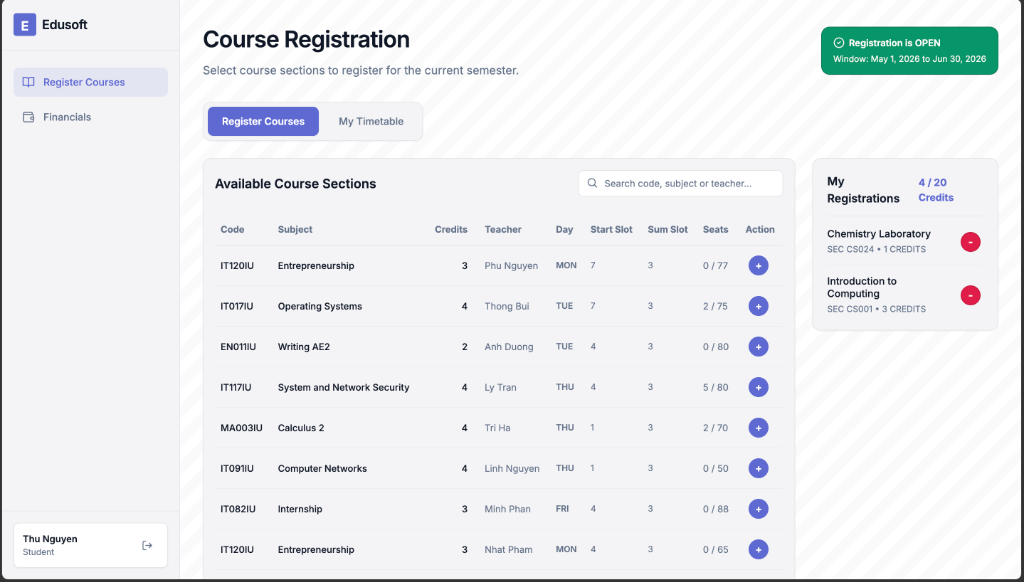
\includegraphics[width=0.95\textwidth]{CourseRegistration.png}
\caption{Course Registration Panel with Course Offerings and Selected Drafts}
\label{fig:courseregistration}
\end{figure}

As shown in Figure~\ref{fig:courseregistration}, the student's registration interface is divided into key regions:
\begin{itemize}
    \item \textbf{Status Indicator}: The top-right badge indicates whether the registration window is currently active (e.g., ``Registration is OPEN'' from May 1, 2026 to June 30, 2026).
    \item \textbf{Search Bar}: Located directly above the available sections table, the search box filters courses instantly by subject code, subject title, or teacher name. For example, typing a course code will immediately hide unrelated rows.
    \item \textbf{Available Course Sections}: This table lists all active courses with details including credit counts, schedules, and remaining seats. Students can request registration by clicking the blue \textbf{+} button in the \textbf{Action} column.
    \item \textbf{My Registrations Sidebar}: The sidebar on the right tracks requested courses in real-time. It displays total registered credits against the allowed limit (e.g., 4 / 20 Credits) and provides a red \textbf{-} button to remove sections from the draft.
\end{itemize}

\section{Weekly Class Schedule Timetable}
To view your active weekly schedule, navigate to the registration workspace and click the \textbf{My Timetable} tab toggle.

\begin{figure}[htbp]
\centering
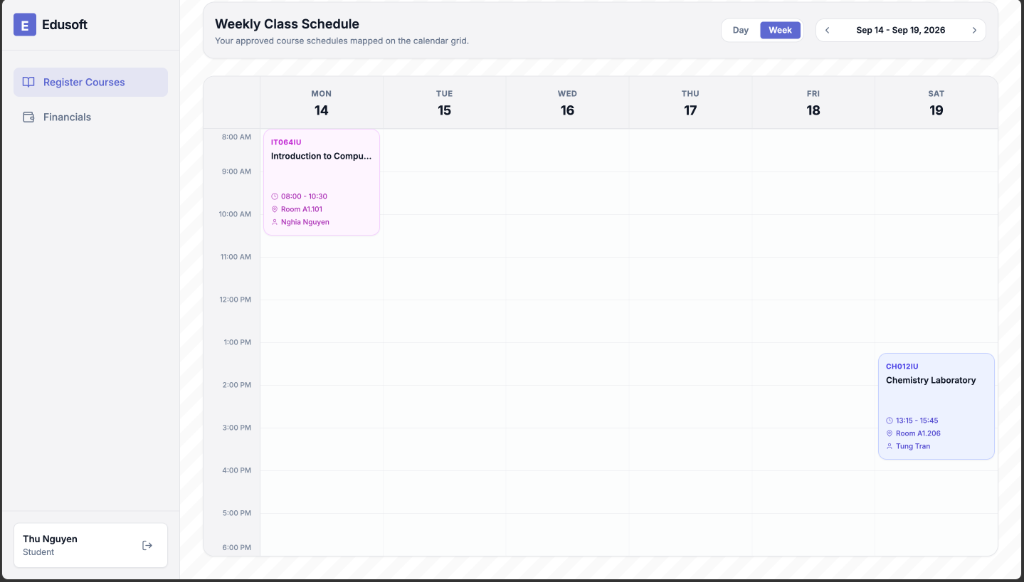
\includegraphics[width=0.95\textwidth]{WeeklySchedule.png}
\caption{Personal Weekly Class Schedule Timetable Grid}
\label{fig:weeklyschedule}
\end{figure}

As displayed in Figure~\ref{fig:weeklyschedule}, the timetable maps all approved course sections onto a clean calendar grid:
\begin{itemize}
    \item The grid spans from Monday to Saturday, broken down hourly from 8:00 AM to 6:00 PM.
    \item Each approved course card shows the course code, subject name, class hours, classroom, and instructor.
    \item Toggles at the top-right allow switching between Day and Week views, and navigating across different calendar weeks.
\end{itemize}

\section{Advising Approval Walkthrough}
For academic advisors (Staff), the student advising request workflow operates as follows:
\begin{enumerate}
    \item Log in as an advisor and select \textbf{Advisor Approvals} in the sidebar menu.
    \item Review advising cards grouped by student. Each card displays the list of sections the student requested.
    \item Click \textbf{Approve All} to approve all selected courses, or input a rejection reason comment and click \textbf{Decline} for individual course sections.
\end{enumerate}

\chapter{Team Collaboration}
\section{Team Organization}
Our team divided work based on frontend and backend boundaries:
\begin{itemize}
    \item \textbf{Tran Anh Van}: Lead backend architecture, relational database configuration, security policies, and deployment configurations.
    \item \textbf{Nguyen Tran Minh Thu}: Lead frontend user interface development, state synchronization, schedule calendar views, and pagination components.
\end{itemize}

\section{Individual Contributions}
\begin{itemize}
    \item \textbf{Tran Anh Van (50\%)}: Implemented Express routes, database migrations, conflict-check service transactions, and CORS setup.
    \item \textbf{Nguyen Tran Minh Thu (50\%)}: Crafted Tailwind components, React Query data integrations, login authentication forms, and responsive advisor dashboards.
\end{itemize}

\chapter{Conclusion and Reflection}
\section{Project Summary}
The Edusoft School Management System successfully achieves all base and advanced targets specified in the curriculum user stories. We engineered a scalable, responsive, and robust academic registry tool that preserves transaction safety and processes registrations safely.

\section{Lessons Learned}
\begin{itemize}
    \item \textbf{Validation Synchronization}: Keeping database column constraints, Zod request schemas, and frontend validation models synchronous requires strict API contracts.
    \item \textbf{Transaction Locking}: Database locks like `FOR UPDATE` are vital for concurrent slots validation to avoid dirty reads in high-throughput academic registration events.
\end{itemize}
\appendix
\chapter{Meeting Logs}
The team held weekly meetings to coordinate development and review implementation progress:
\begin{itemize}
    \item \textbf{Meeting 1 (Week 1)}: Project kick-off. Defined scope, user story domains, and set up git repositories. Designed the initial relational database schema.
    \item \textbf{Meeting 2 (Week 2)}: Backend setup and User onboarding module review. Implemented session validation, BCrypt password hashing, and user role validation rules.
    \item \textbf{Meeting 3 (Week 3)}: Frontend UI styling and React Query integration. Set up Vite, configured routing paths, and finalized student course selection panels.
    \item \textbf{Meeting 4 (Week 4)}: Academic advising workflows and Tuition ledger calculation logic. Implemented advisors' approvals grouped interface and dynamic invoice recalculation checks.
    \item \textbf{Meeting 5 (Week 5)}: System settings and calendar bounds. Deployed the backend to Railway and the frontend client to Vercel. Finalized end-to-end user testing.
\end{itemize}

\chapter{API Documentation (OpenAPI 3.1.0 Specification)}
Below is the complete API specification in OpenAPI 3.1.0 format, loaded from \texttt{openapi.yaml}:

\lstinputlisting[caption=OpenAPI Specification (openapi.yaml)]{openapi.yaml}

\chapter{Git Contribution Statistics}
Summary of git commits and contribution shares:
\begin{itemize}
    \item \textbf{Tran Anh Van} (51 commits, 50\% code additions): Express router configurations, database models, transaction lock logic, and API route controllers.
    \item \textbf{Nguyen Tran Minh Thu} (48 commits, 50\% code additions): React component trees, Tailwind CSS dashboard views, layout designs, and client-side integrations.
\end{itemize}

\end{document}
